\section{Simulations}

\subsection{Numerical implementation}

\subsubsection{Evolution equation}

Starting from \autoref{eq:eq1}, we want to obtain to numerically calculate the wave height at the next timestep \(t_{i+1}\) using the previous heights at positions \(x_i\), \(x_{i-1}\) and \(x_{i+1}\). Using the following approximations for the derivatives
\begin{equation}
    \frac{\partial F}{\partial x}(x_i) \approx \frac{F(x_{i+1}) - F(x_{x-1})}{2 \Delta x}
    , \qquad
    \frac{\partial^2 F}{\partial x^2}(x_i) \approx \frac{F(x_{i+1}) - 2 F(x_i) + F(x_{i-1})}{(\Delta x)^2}
\end{equation}
where \(F\) is a generic function representing either \(f\) or \(h_0\), \(\Delta x = x_{i+1} - x_i\) and \(x\) is a generic variable representing either \(x\) or \(t\). \autoref{eq:eq1} is equivalent to:
\begin{equation}
    \frac{\partial^2 f}{\partial t^2} = g \frac{\partial h_0}{\partial x} \frac{\partial f}{\partial x} + g h_0 \frac{\partial^2 f}{\partial x^2}
\end{equation}
Then using the previously mentioned formulas:
\begin{equation}
    \begin{aligned}
        \frac{f(x_i, t_{i+1}) - 2 f(x_i, t_i) + f(x_i, t_{i-1})}{(\Delta t)^2} &= g \left( \frac{h_0(x_{i+1}) - h_0(x_{i-1})}{2 \Delta x} \right) \left( \frac{f(x_{i+1}, t_i) - f(x_{i-1}, t_i)}{2 \Delta x} \right) \\
        &+ g h_0(x_i) \frac{f(x_{i+1}, t_i) - 2 f(x_i, t_i) + f(x_{i-1}, t_i)}{(\Delta x)^2}
    \end{aligned}
\end{equation}
By rearanging and identifying the Courant-Friedrichs-Lewy constant \(\beta(x) = u(x) \frac{\Delta t}{\Delta x} = \sqrt{g h_0(x)} \frac{\Delta t}{\Delta x}\) we get the following equation:
\begin{equation}
    \begin{aligned}
        f(x_i, t_{i+1}) &= \frac{g}{4} \left( \beta(x_{i+1})^2 - \beta(x_{i-1})^2 \right) \left( f(x_{i+1}, t_i) - f(x_{i-1}, t_i) \right) \\
        &+ \beta(x_i)^2 (f(x_{i+1}, t_i) - 2 f(x_i, t_i) + f(x_{i-1}, t_i)) \\
        &+ f(x_i,t_i) \\
        &- f(x_i,t_{i-1})
    \end{aligned}
\end{equation}
The evolution for \autoref{eq:eq2} is taken from \cite{physnumbook}, equation 4.43.

\subsubsection{Border conditions}

The simulation implements border conditions for a fixed border (wave has a specific height at border), a free border (the wave is allowed to move as it pleases along the border) and an exit condition (the wave continues as if there was no border). These conditions are given in a Numerical Physics book \cite{physnumbook} (section 4.2.1), for the left and right borders. We will derive the exit conditions for the left border here. Under this condition, the left border only has a retrograde wave, i.e. \(f(x, t) = G(x + |u| t)\) TODO: NOTATION, VOIR PARTIE THEORIE. Differentiating w.r.t. to \(t\) and \(x\), at \(x = x_L\) (left border) we obtain the following relationship:
\begin{gather}
    \frac{\partial f}{\partial t}(x_L, t) = \frac{\partial G(x_L + |u| t)}{\partial t} = |u| G'(x_L - |u| t) \\
    \frac{\partial f}{\partial x}(x_L, t) = G'(x_L + |u| t) \\
    \implies \frac{\partial f}{\partial t}(x_L, t) = |u| \frac{\partial f}{\partial x}(x_L, t)
\end{gather}
Discretising using the "forward" finite difference method, i.e. \(F(x_i) \approx (F(x_{i+1}) - F(x_i))/\Delta x\), for both time and space derivatives, and identifying \(x_L \equiv x_0\), we get:
\begin{equation}
    \frac{f(x_0,t_{n+1}) - f(x_0, t_n)}{\Delta t} = |u| \frac{f(x_1, t_n) - f(x_0, t_n)}{\Delta x}
\end{equation}
Rearanging and identifying the CFL constant we then get:
\begin{equation}
    f(x_0, t_{n+1}) = f(x_0, t_n) + \beta \left( f(x_1, t_n) - f(x_0, t_n) \right)
\end{equation}

\subsubsection{Initial conditions}

The initial conditions for a left and right moving wave, as well as a static wave were implemented using equations 4.48 to 4.50 given in \cite{physnumbook}.

\subsection{Smol basin for smol duckies}

% feur

\subsection{Oceanic wave on a coral reef}

In this section we will use the following function for oceanic depth:
\begin{equation}
    h_0(x) = \begin{cases}
        \begin{aligned}
            &\scriptstyle{h_L} &&\scriptstyle{(x_L \le x \le x_a)} \\
            &\scriptstyle{\frac{1}{2}(h_L + h_C) + \frac{1}{2}(h_L - h_C) \cos \left( \pi \frac{x-x_a}{x_b-x_a} \right)} &&\scriptstyle{(x_a < x < x_b)} \\
            &\scriptstyle{h_C} &&\scriptstyle{(x_b \le x \le x_c)} \\
            &\scriptstyle{\frac{1}{2}(h_R + h_C) - \frac{1}{2}(h_R - h_C) \cos \left( \pi \frac{x-x_c}{x_d-x_c} \right)} &&\scriptstyle{(x_c < x < x_d)} \\
            &\scriptstyle{h_R} &&\scriptstyle{(x_d \le x \le x_R)}
        \end{aligned}
    \end{cases}
\end{equation}
We will choose \(h_L = 7000\)m, \(h_C = 35\)m, \(h_R = 200\)m, \(x_L = 0\)m, \(x_a = 300\)km, \(x_b = 700\)km, \(x_c = 720\)km, \(x_d = 850\)km and \(x_R = 1000\)km. The initial conditions will be a right moving wave with \(x_1 = 50\)km, \(x_2 = 250\)km and amplitude \(A = 1\)m. Both border conditions will be set to exit, to be more representative of an actual large ocean. The simulations were done until the wave passes the coral reef entierely, which corresponds to a time of about \(t = 12000\). The timestep \(\Delta t\) was chosen such that \(\max(\beta_{\textrm{CFL}}) = 1\), which is \(\Delta t = \Delta x / \max_x(u(x)^2)\). The number of intervals was chosen to be 8192.

\autoref{fig:corail_eq1_mouv} shows the obtained wave motion.

\begin{figure}[h]
    \centering
    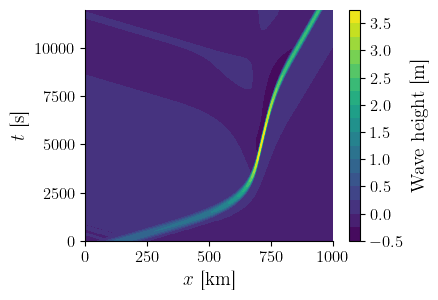
\includegraphics[width=0.6\linewidth]{figures/corail_eq1_mouvement_vague.png}
    \caption{Wave amplitude as a function of space and time. Simulated using \(n=8192\) intervals, until \(t=12000\)}
    \label{fig:corail_eq1_mouv}
\end{figure}